% Options for packages loaded elsewhere
\PassOptionsToPackage{unicode}{hyperref}
\PassOptionsToPackage{hyphens}{url}
%
\documentclass[
]{article}
\usepackage{amsmath,amssymb}
\usepackage{lmodern}
\usepackage{ifxetex,ifluatex}
\ifnum 0\ifxetex 1\fi\ifluatex 1\fi=0 % if pdftex
  \usepackage[T1]{fontenc}
  \usepackage[utf8]{inputenc}
  \usepackage{textcomp} % provide euro and other symbols
\else % if luatex or xetex
  \usepackage{unicode-math}
  \defaultfontfeatures{Scale=MatchLowercase}
  \defaultfontfeatures[\rmfamily]{Ligatures=TeX,Scale=1}
\fi
% Use upquote if available, for straight quotes in verbatim environments
\IfFileExists{upquote.sty}{\usepackage{upquote}}{}
\IfFileExists{microtype.sty}{% use microtype if available
  \usepackage[]{microtype}
  \UseMicrotypeSet[protrusion]{basicmath} % disable protrusion for tt fonts
}{}
\makeatletter
\@ifundefined{KOMAClassName}{% if non-KOMA class
  \IfFileExists{parskip.sty}{%
    \usepackage{parskip}
  }{% else
    \setlength{\parindent}{0pt}
    \setlength{\parskip}{6pt plus 2pt minus 1pt}}
}{% if KOMA class
  \KOMAoptions{parskip=half}}
\makeatother
\usepackage{xcolor}
\IfFileExists{xurl.sty}{\usepackage{xurl}}{} % add URL line breaks if available
\IfFileExists{bookmark.sty}{\usepackage{bookmark}}{\usepackage{hyperref}}
\hypersetup{
  pdftitle={module5\_Estes},
  pdfauthor={Andrew Estes},
  hidelinks,
  pdfcreator={LaTeX via pandoc}}
\urlstyle{same} % disable monospaced font for URLs
\usepackage[margin=1in]{geometry}
\usepackage{color}
\usepackage{fancyvrb}
\newcommand{\VerbBar}{|}
\newcommand{\VERB}{\Verb[commandchars=\\\{\}]}
\DefineVerbatimEnvironment{Highlighting}{Verbatim}{commandchars=\\\{\}}
% Add ',fontsize=\small' for more characters per line
\usepackage{framed}
\definecolor{shadecolor}{RGB}{248,248,248}
\newenvironment{Shaded}{\begin{snugshade}}{\end{snugshade}}
\newcommand{\AlertTok}[1]{\textcolor[rgb]{0.94,0.16,0.16}{#1}}
\newcommand{\AnnotationTok}[1]{\textcolor[rgb]{0.56,0.35,0.01}{\textbf{\textit{#1}}}}
\newcommand{\AttributeTok}[1]{\textcolor[rgb]{0.77,0.63,0.00}{#1}}
\newcommand{\BaseNTok}[1]{\textcolor[rgb]{0.00,0.00,0.81}{#1}}
\newcommand{\BuiltInTok}[1]{#1}
\newcommand{\CharTok}[1]{\textcolor[rgb]{0.31,0.60,0.02}{#1}}
\newcommand{\CommentTok}[1]{\textcolor[rgb]{0.56,0.35,0.01}{\textit{#1}}}
\newcommand{\CommentVarTok}[1]{\textcolor[rgb]{0.56,0.35,0.01}{\textbf{\textit{#1}}}}
\newcommand{\ConstantTok}[1]{\textcolor[rgb]{0.00,0.00,0.00}{#1}}
\newcommand{\ControlFlowTok}[1]{\textcolor[rgb]{0.13,0.29,0.53}{\textbf{#1}}}
\newcommand{\DataTypeTok}[1]{\textcolor[rgb]{0.13,0.29,0.53}{#1}}
\newcommand{\DecValTok}[1]{\textcolor[rgb]{0.00,0.00,0.81}{#1}}
\newcommand{\DocumentationTok}[1]{\textcolor[rgb]{0.56,0.35,0.01}{\textbf{\textit{#1}}}}
\newcommand{\ErrorTok}[1]{\textcolor[rgb]{0.64,0.00,0.00}{\textbf{#1}}}
\newcommand{\ExtensionTok}[1]{#1}
\newcommand{\FloatTok}[1]{\textcolor[rgb]{0.00,0.00,0.81}{#1}}
\newcommand{\FunctionTok}[1]{\textcolor[rgb]{0.00,0.00,0.00}{#1}}
\newcommand{\ImportTok}[1]{#1}
\newcommand{\InformationTok}[1]{\textcolor[rgb]{0.56,0.35,0.01}{\textbf{\textit{#1}}}}
\newcommand{\KeywordTok}[1]{\textcolor[rgb]{0.13,0.29,0.53}{\textbf{#1}}}
\newcommand{\NormalTok}[1]{#1}
\newcommand{\OperatorTok}[1]{\textcolor[rgb]{0.81,0.36,0.00}{\textbf{#1}}}
\newcommand{\OtherTok}[1]{\textcolor[rgb]{0.56,0.35,0.01}{#1}}
\newcommand{\PreprocessorTok}[1]{\textcolor[rgb]{0.56,0.35,0.01}{\textit{#1}}}
\newcommand{\RegionMarkerTok}[1]{#1}
\newcommand{\SpecialCharTok}[1]{\textcolor[rgb]{0.00,0.00,0.00}{#1}}
\newcommand{\SpecialStringTok}[1]{\textcolor[rgb]{0.31,0.60,0.02}{#1}}
\newcommand{\StringTok}[1]{\textcolor[rgb]{0.31,0.60,0.02}{#1}}
\newcommand{\VariableTok}[1]{\textcolor[rgb]{0.00,0.00,0.00}{#1}}
\newcommand{\VerbatimStringTok}[1]{\textcolor[rgb]{0.31,0.60,0.02}{#1}}
\newcommand{\WarningTok}[1]{\textcolor[rgb]{0.56,0.35,0.01}{\textbf{\textit{#1}}}}
\usepackage{graphicx}
\makeatletter
\def\maxwidth{\ifdim\Gin@nat@width>\linewidth\linewidth\else\Gin@nat@width\fi}
\def\maxheight{\ifdim\Gin@nat@height>\textheight\textheight\else\Gin@nat@height\fi}
\makeatother
% Scale images if necessary, so that they will not overflow the page
% margins by default, and it is still possible to overwrite the defaults
% using explicit options in \includegraphics[width, height, ...]{}
\setkeys{Gin}{width=\maxwidth,height=\maxheight,keepaspectratio}
% Set default figure placement to htbp
\makeatletter
\def\fps@figure{htbp}
\makeatother
\setlength{\emergencystretch}{3em} % prevent overfull lines
\providecommand{\tightlist}{%
  \setlength{\itemsep}{0pt}\setlength{\parskip}{0pt}}
\setcounter{secnumdepth}{-\maxdimen} % remove section numbering
\ifluatex
  \usepackage{selnolig}  % disable illegal ligatures
\fi

\title{module5\_Estes}
\author{Andrew Estes}
\date{9/25/2021}

\begin{document}
\maketitle

\begin{enumerate}
\def\labelenumi{\arabic{enumi}.}
\tightlist
\item
  This first problem will have you explore the AmesHousing data set in
  order to discover why we had to limit our use of data to homes built
  on or after 1950.
\end{enumerate}

\begin{enumerate}
\def\labelenumi{\alph{enumi}.}
\tightlist
\item
  First, let's look at what we would have found if we hadn't looked only
  at homes built after 1950. Write some code to • load the AmesHousing
  data set into R and create the data frame ames, • create a new column
  called Remodeled, as we did in the lecture notes, that will be true if
  Year\_Built != Year\_Remod\_Add, • sample 500 data points from the
  ames data frame, using set.seed(248) to make sure we all get the same
  sample, and • run an independent-sample t-test to test whether the
  means of the remodeled and nonremodeled groups are different.
\end{enumerate}

\begin{Shaded}
\begin{Highlighting}[]
\FunctionTok{library}\NormalTok{(AmesHousing)}
\end{Highlighting}
\end{Shaded}

\begin{verbatim}
## Warning: package 'AmesHousing' was built under R version 4.1.1
\end{verbatim}

\begin{Shaded}
\begin{Highlighting}[]
\FunctionTok{library}\NormalTok{(tidyverse)}
\end{Highlighting}
\end{Shaded}

\begin{verbatim}
## -- Attaching packages --------------------------------------- tidyverse 1.3.1 --
\end{verbatim}

\begin{verbatim}
## v ggplot2 3.3.5     v purrr   0.3.4
## v tibble  3.1.3     v dplyr   1.0.7
## v tidyr   1.1.3     v stringr 1.4.0
## v readr   2.0.0     v forcats 0.5.1
\end{verbatim}

\begin{verbatim}
## Warning: package 'tidyr' was built under R version 4.1.1
\end{verbatim}

\begin{verbatim}
## -- Conflicts ------------------------------------------ tidyverse_conflicts() --
## x dplyr::filter() masks stats::filter()
## x dplyr::lag()    masks stats::lag()
\end{verbatim}

\begin{Shaded}
\begin{Highlighting}[]
\FunctionTok{library}\NormalTok{(ggplot2)}
\FunctionTok{library}\NormalTok{(tinytex)}
\NormalTok{Ames }\OtherTok{\textless{}{-}} \FunctionTok{make\_ames}\NormalTok{()}

\NormalTok{Ames}\FloatTok{.50} \OtherTok{\textless{}{-}}\NormalTok{ Ames }\SpecialCharTok{\%\textgreater{}\%}
  \FunctionTok{filter}\NormalTok{(Ames}\SpecialCharTok{$}\NormalTok{Year\_Built }\SpecialCharTok{\textgreater{}=} \DecValTok{1950}\NormalTok{)}

\NormalTok{Ames2 }\OtherTok{\textless{}{-}}\NormalTok{ Ames }\SpecialCharTok{\%\textgreater{}\%} 
  \FunctionTok{mutate}\NormalTok{(}\AttributeTok{Remodeled =}\NormalTok{ Ames}\SpecialCharTok{$}\NormalTok{Year\_Built }\SpecialCharTok{!=}\NormalTok{ Ames}\SpecialCharTok{$}\NormalTok{Year\_Remod\_Add)}

\FunctionTok{set.seed}\NormalTok{(}\DecValTok{248}\NormalTok{)}
\FunctionTok{t.test}\NormalTok{(Sale\_Price }\SpecialCharTok{\textasciitilde{}}\NormalTok{ Remodeled, }\AttributeTok{data=}\NormalTok{Ames2)}
\end{Highlighting}
\end{Shaded}

\begin{verbatim}
## 
##  Welch Two Sample t-test
## 
## data:  Sale_Price by Remodeled
## t = 2.5372, df = 2726.7, p-value = 0.01123
## alternative hypothesis: true difference in means between group FALSE and group TRUE is not equal to 0
## 95 percent confidence interval:
##   1719.841 13421.938
## sample estimates:
## mean in group FALSE  mean in group TRUE 
##            184312.8            176741.9
\end{verbatim}

\begin{enumerate}
\def\labelenumi{\alph{enumi}.}
\setcounter{enumi}{1}
\tightlist
\item
  Compare the results of this t-test to those shown in the lecture
  notes. There should be one aspect that's markedly different.
\end{enumerate}

\begin{Shaded}
\begin{Highlighting}[]
\CommentTok{\#The mean group in TRUE is very different: 176k vs 206k}
\end{Highlighting}
\end{Shaded}

\begin{enumerate}
\def\labelenumi{\alph{enumi}.}
\setcounter{enumi}{2}
\tightlist
\item
  What's going on? Make a plot that helps you explore the data. Then
  write a brief explanation of why the results differ, depending on
  whether homes built before 1950 are included in the data set. {[}Hint:
  There might be lots of ways to do this, but a scatter plot involving
  Year\_Remod\_Add and Year\_Built might work well.{]}
\end{enumerate}

\begin{Shaded}
\begin{Highlighting}[]
\NormalTok{oneC }\OtherTok{\textless{}{-}} 
  \FunctionTok{ggplot}\NormalTok{() }\SpecialCharTok{+}
  \FunctionTok{geom\_point}\NormalTok{(}\AttributeTok{data=}\NormalTok{Ames}\FloatTok{.50}\NormalTok{, }\FunctionTok{aes}\NormalTok{(Sale\_Price}\SpecialCharTok{/}\DecValTok{1000}\NormalTok{, Year\_Remod\_Add, }\AttributeTok{color=}\StringTok{"lightred"}\NormalTok{)) }\SpecialCharTok{+}
  \FunctionTok{geom\_point}\NormalTok{(}\AttributeTok{data=}\NormalTok{Ames2, }\FunctionTok{aes}\NormalTok{(Sale\_Price}\SpecialCharTok{/}\DecValTok{1000}\NormalTok{,  Year\_Built, }\AttributeTok{color=}\StringTok{"darkblue"}\NormalTok{))}
\NormalTok{oneC }\SpecialCharTok{+} \FunctionTok{coord\_flip}\NormalTok{()}
\end{Highlighting}
\end{Shaded}

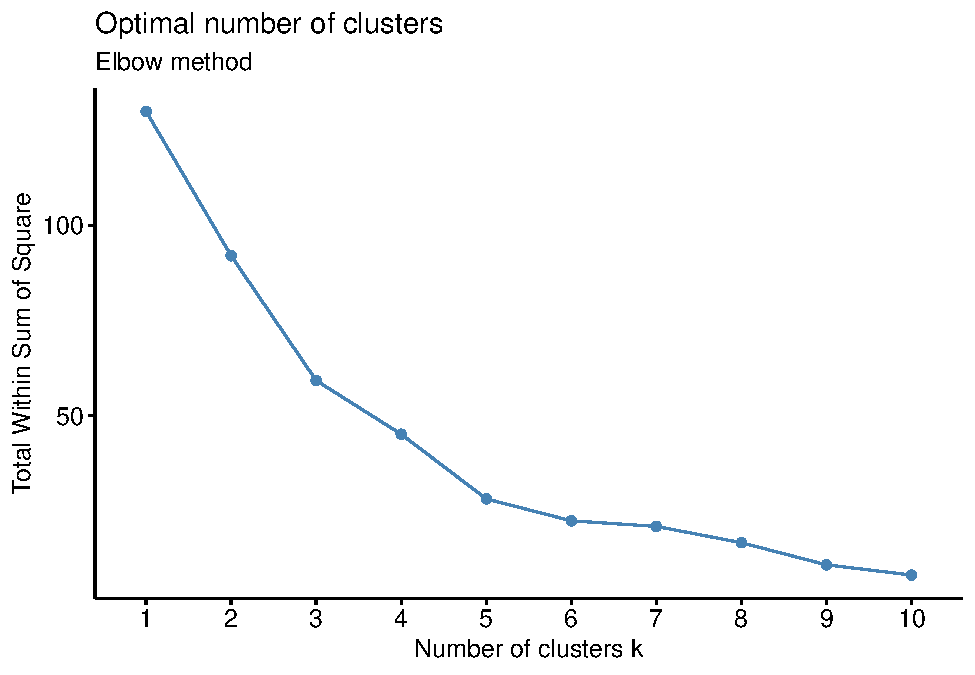
\includegraphics{homework5_Estes_files/figure-latex/unnamed-chunk-3-1.pdf}

\begin{Shaded}
\begin{Highlighting}[]
\CommentTok{\#A recently remodeled home offers more value than a home that was remodeled 70+ years ago}
\CommentTok{\#New houses are priced similarly to recently remodeld homes}
\end{Highlighting}
\end{Shaded}

\begin{enumerate}
\def\labelenumi{\arabic{enumi}.}
\setcounter{enumi}{1}
\tightlist
\item
  In this problem, we'll look at simulating the results of an
  independent-sample t-test in order to gain some insight about sample
  sizes.
\end{enumerate}

\begin{enumerate}
\def\labelenumi{\alph{enumi}.}
\tightlist
\item
  Complete the code stub below to write code to generate two sets of
  random, normallydistributed data, with the sample sizes, means and
  standard deviations as specified in the code. Then perform an
  independent-sample t-test using your two samples as the two groups to
  be compared. {[}Note: we're purposefully not going to use set.seed
  here.{]}
\end{enumerate}

\begin{Shaded}
\begin{Highlighting}[]
\NormalTok{n1 }\OtherTok{\textless{}{-}} \DecValTok{200}
\NormalTok{n2 }\OtherTok{\textless{}{-}} \DecValTok{200}
\NormalTok{mu1 }\OtherTok{\textless{}{-}} \DecValTok{15}
\NormalTok{mu2 }\OtherTok{\textless{}{-}} \DecValTok{17}
\NormalTok{sigma1 }\OtherTok{\textless{}{-}} \DecValTok{8}
\NormalTok{sigma2 }\OtherTok{\textless{}{-}} \DecValTok{8}

\NormalTok{first }\OtherTok{\textless{}{-}} \FunctionTok{rnorm}\NormalTok{(n1, }\AttributeTok{mean =}\NormalTok{ mu1, }\AttributeTok{sd =}\NormalTok{ sigma1)}
\NormalTok{second }\OtherTok{\textless{}{-}} \FunctionTok{rnorm}\NormalTok{(n2, }\AttributeTok{mean =}\NormalTok{ mu2, }\AttributeTok{sd =}\NormalTok{ sigma2)}
\FunctionTok{t.test}\NormalTok{(first, second, }\AttributeTok{alternative =} \StringTok{"two.sided"}\NormalTok{, }\AttributeTok{paired =} \ConstantTok{FALSE}\NormalTok{, }\AttributeTok{var.equal =} \ConstantTok{FALSE}\NormalTok{)}
\end{Highlighting}
\end{Shaded}

\begin{verbatim}
## 
##  Welch Two Sample t-test
## 
## data:  first and second
## t = -3.9182, df = 397.79, p-value = 0.000105
## alternative hypothesis: true difference in means is not equal to 0
## 95 percent confidence interval:
##  -4.860058 -1.612484
## sample estimates:
## mean of x mean of y 
##  14.20690  17.44317
\end{verbatim}

\begin{Shaded}
\begin{Highlighting}[]
\FunctionTok{t.test}\NormalTok{(first, second, }\AttributeTok{alternative =} \StringTok{"two.sided"}\NormalTok{, }\AttributeTok{paired =} \ConstantTok{TRUE}\NormalTok{, }\AttributeTok{var.equal =} \ConstantTok{FALSE}\NormalTok{)}
\end{Highlighting}
\end{Shaded}

\begin{verbatim}
## 
##  Paired t-test
## 
## data:  first and second
## t = -3.9611, df = 199, p-value = 0.0001039
## alternative hypothesis: true difference in means is not equal to 0
## 95 percent confidence interval:
##  -4.847404 -1.625138
## sample estimates:
## mean of the differences 
##               -3.236271
\end{verbatim}

\begin{enumerate}
\def\labelenumi{\alph{enumi}.}
\setcounter{enumi}{1}
\tightlist
\item
  Suppose your simulated data represents the results of a trial of a new
  blood pressure medication. Group 1 represents the decrease in blood
  pressure for a group taking the current ``best in class'' medication,
  while Group 2 represents the decrease in blood pressure for a group
  taking a new competitor's drug. Interpret the results of the test you
  did in a way that communicates accurately, but without unnecessary
  complexity. Make sure that you refer to the specifics of this
  real-world scenario. {[}Assume α = .05 so that you can get a specific
  Yes/No answer to the test.{]}
\end{enumerate}

\begin{Shaded}
\begin{Highlighting}[]
\CommentTok{\#Comparing the two samples, there is a statistically significant difference between the two groups.}
\CommentTok{\#With a p{-}value of .01485, it is a strongly correlated. }
\CommentTok{\#Group 1 is not as successful, on average, at reducing the BP as Group 2}
\end{Highlighting}
\end{Shaded}

\begin{enumerate}
\def\labelenumi{\arabic{enumi}.}
\setcounter{enumi}{2}
\tightlist
\item
  This question picks up where the last left off. If you run your code
  from Question 2 several times (click the green arrow on the code chunk
  several times), you should notice that sometimes you get a p-value
  that would reject the null hypothesis, and sometimes you don't.
  Furthermore, remember that there are two ways that a hypothesis test
  might be in error: • Type I Error: Rejecting H0 when H0 is really
  true. Prob(Type I) = α. • Type II Error: Failing to reject H0 when H0
  is really false. Prob(Type II) = β. We can control the probability of
  committing a Type I error by controlling the significance level, α,
  that we choose for the test. On the other hand, calculating and
  controlling β is harder. Even calculating β requires an assumption
  about what we think the true alternative really is. Not just μ2 − μ1 ≠
  0, but, for example, μ2 − μ1 = 2. With that assumption, it is possible
  to calculate β. This can be done theoretically, or---as we'll
  see---through simulation.
\end{enumerate}

\begin{enumerate}
\def\labelenumi{\alph{enumi}.}
\tightlist
\item
  By setting mu1 \textless- 15 and mu2 \textless- 17 in the code above,
  we've actually made the assumption in this simulation that the true
  population means are not equal---in fact, they differ by 2. Therefore,
  to get an estimate of β, all we need to do is to run the simulations
  and hypothesis test many times, and look at the percentage of times
  that we fail to reject the null hypothesis, even though we know that
  the null hypotheses is false in our simulation. Run your simulation
  and t-test code many times (maybe at least 20 times?), and calculate
  the percentage of those runs where you fail to reject the null
  hypothesis. Then fill in the sentence below: ``Under the assumption
  that the new drug lowers blood pressure by 2 mmHg more than its
  competitor, I estimate the the probability of failing to detect that
  difference is
  \_\_\_\_\_\_\_\_\_\_\_\_\_\_\_\_\_\_\_\_\_\_\_\_\_\_\_.''
\end{enumerate}

\begin{Shaded}
\begin{Highlighting}[]
\CommentTok{\#“Under the assumption that the new drug lowers blood pressure by 2 mmHg more}
\CommentTok{\#than its competitor, I estimate the probability of failing to detect that difference is}
\CommentTok{\#70\% (ran 20 times, 14 results were not statistically significant)}
\end{Highlighting}
\end{Shaded}

\begin{enumerate}
\def\labelenumi{\alph{enumi}.}
\setcounter{enumi}{1}
\tightlist
\item
  Suppose you find this probability of Type II error to be too high in
  the scenario outlined above. One way to decrease it would be to raise
  your sample size. By experimenting with changing n1 and n2, find the
  minimum sample sizes necessary to reduce your probability of Type II
  error to 5\%. {[}You might try n = 100, n = 200, etc. as a start.
  Note: The power of a test is defined to be 1 − β, so we're really
  finding the sample size that would give a power of 95\% for this
  test.{]}
\end{enumerate}

\begin{Shaded}
\begin{Highlighting}[]
\CommentTok{\#Changed the N value to 300, then to 100, then to 200}
\end{Highlighting}
\end{Shaded}

\begin{enumerate}
\def\labelenumi{\arabic{enumi}.}
\setcounter{enumi}{3}
\tightlist
\item
  We saw that taking the log transform of Sale\_Price was one way to try
  to get control of the variance of residuals in our simple linear
  regression. Another way to try to improve the model's fit and the
  model assumptions is to add further important variables to the model.
  Often bad fit is the result of confounding from lurking variables. In
  this problem, start with the first multiple linear regression model we
  looked at in the lecture. It's named fit.original in the code chunk
  below. Then do the following:
\end{enumerate}

\begin{enumerate}
\def\labelenumi{\alph{enumi}.}
\tightlist
\item
  Write code to plot residuals vs.~fit for fit.original (try to find the
  right plot option to print out only that graph).
\end{enumerate}

\begin{Shaded}
\begin{Highlighting}[]
\NormalTok{fit.original }\OtherTok{\textless{}{-}} \FunctionTok{lm}\NormalTok{(Sale\_Price }\SpecialCharTok{\textasciitilde{}}\NormalTok{ Year\_Built }\SpecialCharTok{+}\NormalTok{ First\_Flr\_SF, }\AttributeTok{data=}\NormalTok{Ames)}
\NormalTok{fit.sale.year }\OtherTok{\textless{}{-}} \FunctionTok{lm}\NormalTok{(Sale\_Price }\SpecialCharTok{\textasciitilde{}}\NormalTok{ Year\_Built, }\AttributeTok{data=}\NormalTok{Ames)}
\FunctionTok{plot}\NormalTok{(fit.sale.year)}
\end{Highlighting}
\end{Shaded}

\includegraphics{homework5_Estes_files/figure-latex/unnamed-chunk-8-1.pdf}
\includegraphics{homework5_Estes_files/figure-latex/unnamed-chunk-8-2.pdf}
\includegraphics{homework5_Estes_files/figure-latex/unnamed-chunk-8-3.pdf}
\includegraphics{homework5_Estes_files/figure-latex/unnamed-chunk-8-4.pdf}

\begin{Shaded}
\begin{Highlighting}[]
\FunctionTok{plot}\NormalTok{(fit.original)}
\end{Highlighting}
\end{Shaded}

\includegraphics{homework5_Estes_files/figure-latex/unnamed-chunk-8-5.pdf}
\includegraphics{homework5_Estes_files/figure-latex/unnamed-chunk-8-6.pdf}
\includegraphics{homework5_Estes_files/figure-latex/unnamed-chunk-8-7.pdf}
\includegraphics{homework5_Estes_files/figure-latex/unnamed-chunk-8-8.pdf}

\begin{enumerate}
\def\labelenumi{\alph{enumi}.}
\setcounter{enumi}{1}
\tightlist
\item
  Write code to output the R2-adjusted for fit.original.
\end{enumerate}

\begin{Shaded}
\begin{Highlighting}[]
\FunctionTok{summary}\NormalTok{(fit.original)}
\end{Highlighting}
\end{Shaded}

\begin{verbatim}
## 
## Call:
## lm(formula = Sale_Price ~ Year_Built + First_Flr_SF, data = Ames)
## 
## Residuals:
##     Min      1Q  Median      3Q     Max 
## -434097  -32813   -9218   23910  420116 
## 
## Coefficients:
##                Estimate Std. Error t value Pr(>|t|)    
## (Intercept)  -2.042e+06  6.819e+04  -29.95   <2e-16 ***
## Year_Built    1.068e+03  3.505e+01   30.48   <2e-16 ***
## First_Flr_SF  1.011e+02  2.705e+00   37.39   <2e-16 ***
## ---
## Signif. codes:  0 '***' 0.001 '**' 0.01 '*' 0.05 '.' 0.1 ' ' 1
## 
## Residual standard error: 54540 on 2927 degrees of freedom
## Multiple R-squared:  0.5343, Adjusted R-squared:  0.5339 
## F-statistic:  1679 on 2 and 2927 DF,  p-value: < 2.2e-16
\end{verbatim}

\begin{Shaded}
\begin{Highlighting}[]
\CommentTok{\#adjusted R{-}Squared = 0.5339}
\CommentTok{\#RSE = 54540}
\end{Highlighting}
\end{Shaded}

\begin{enumerate}
\def\labelenumi{\alph{enumi}.}
\setcounter{enumi}{2}
\tightlist
\item
  Think about which variables which variables might also be highly
  related to Sale\_Price. Then create a new model using those variables
  that has a higher R2-adjusted and seems to satisfy the linearity and
  constant variance conditions better. Output the plot of fit
  vs.~residuals and the adjusted r-squared for this new model as well.
  There's no single right answer here---for now you're just playing
  around to see what you'll find.
\end{enumerate}

\begin{Shaded}
\begin{Highlighting}[]
\NormalTok{fit.andrew }\OtherTok{\textless{}{-}} \FunctionTok{lm}\NormalTok{(Sale\_Price }\SpecialCharTok{\textasciitilde{}}\NormalTok{ Year\_Remod\_Add }\SpecialCharTok{+}\NormalTok{ First\_Flr\_SF,}\AttributeTok{data=}\NormalTok{Ames)}
\FunctionTok{summary}\NormalTok{(fit.andrew)}
\end{Highlighting}
\end{Shaded}

\begin{verbatim}
## 
## Call:
## lm(formula = Sale_Price ~ Year_Remod_Add + First_Flr_SF, data = Ames)
## 
## Residuals:
##     Min      1Q  Median      3Q     Max 
## -455250  -32649   -3139   23457  420483 
## 
## Coefficients:
##                  Estimate Std. Error t value Pr(>|t|)    
## (Intercept)    -3.030e+06  9.730e+04  -31.14   <2e-16 ***
## Year_Remod_Add  1.556e+03  4.938e+01   31.51   <2e-16 ***
## First_Flr_SF    1.067e+02  2.629e+00   40.59   <2e-16 ***
## ---
## Signif. codes:  0 '***' 0.001 '**' 0.01 '*' 0.05 '.' 0.1 ' ' 1
## 
## Residual standard error: 54090 on 2927 degrees of freedom
## Multiple R-squared:  0.5419, Adjusted R-squared:  0.5416 
## F-statistic:  1731 on 2 and 2927 DF,  p-value: < 2.2e-16
\end{verbatim}

\begin{Shaded}
\begin{Highlighting}[]
\CommentTok{\#adjusted R{-}Squared = .5416}
\CommentTok{\#RSE = 54090}
\FunctionTok{plot}\NormalTok{(fit.andrew)}
\end{Highlighting}
\end{Shaded}

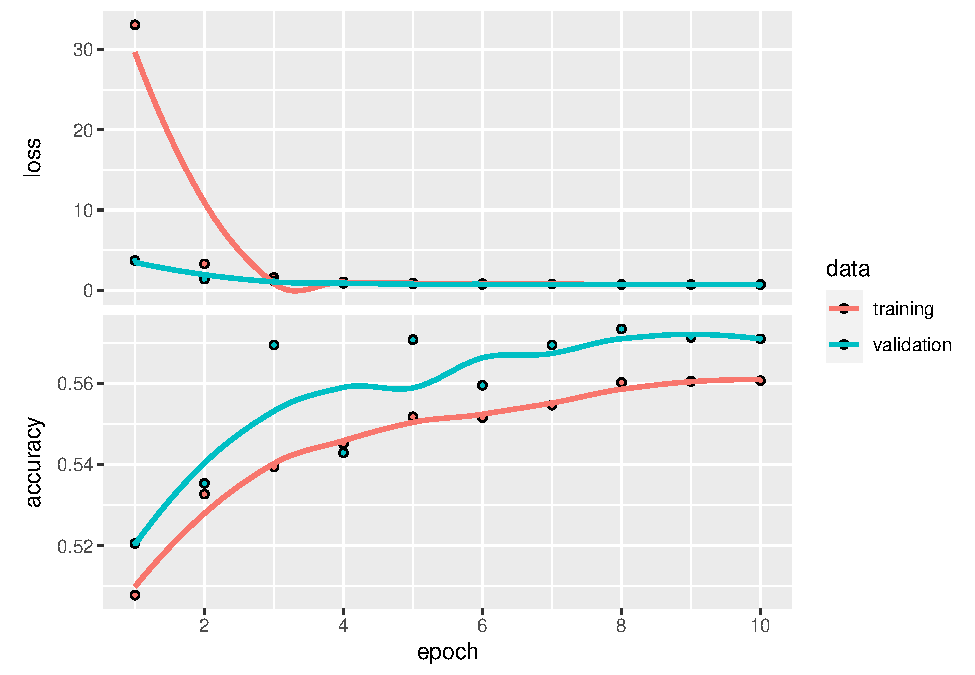
\includegraphics{homework5_Estes_files/figure-latex/unnamed-chunk-10-1.pdf}
\includegraphics{homework5_Estes_files/figure-latex/unnamed-chunk-10-2.pdf}
\includegraphics{homework5_Estes_files/figure-latex/unnamed-chunk-10-3.pdf}
\includegraphics{homework5_Estes_files/figure-latex/unnamed-chunk-10-4.pdf}

\end{document}
